%versi 2 (8-10-2016)
\chapter{Landasan Teori}
\label{chap:teori}

\lstdefinelanguage{JavaScript}{
  keywords={new, true, false, function, return, null, catch, switch, var, if, while, do, else, const, this},
  keywordstyle=\color{blue}\bfseries,
  ndkeywords={moveTo,lineTo,arc},
  ndkeywordstyle=\color{purple}\bfseries,
  identifierstyle=\color{black},
  sensitive=false,
  comment=[l]{//},
  morecomment=[s]{/*}{*/},
  commentstyle=\itshape\color{green},
  stringstyle=\color{red},
  morestring=[b]',
  morestring=[b]",
  captionpos=b,
}

\lstset{
   language=JavaScript,
   backgroundcolor=\color{white},
   extendedchars=true,
   basicstyle=\fontfamily{fvm}\selectfont\small, 
   showstringspaces=false,
   showspaces=false,
   numbers=left,
   numberstyle=\footnotesize,
   numbersep=5pt,
   tabsize=4,
   breaklines=true,
   showtabs=false,
   captionpos=b,
   frame=leftline,
   stepnumber=1,
   literate={-}{-}1{-\,-}{--}1
}

\section{\textit{Snake}}
\label{sec:snake}
\textit{Snake} merupakan permainan mengendalikan ular untuk mendapatkan makanan yang terdapat pada labirin. Dalam permainan ini, pemain mengendalikan ular untuk mendapatkan makanan sebanyak-banyaknya. Setiap ular memakan makanan, maka skor akan bertambah 1 poin dan tubuh ular akan bertambah panjang. Biasanya makanan hanya ada 1 saja pada sebuah labirin. Ketika makanan itu sudah termakan oleh ular, makanan tersebut akan ditempatkan secara acak. Ular dapat bergerak ke atas, bawah, kiri, dan kanan. Namun pada permainan \textit{Snake} yang akan dibuat sekarang, ular dapat bergerak ke segala arah seperti ilustrasi pada Gambar~\ref{fig:ularSegalaArah}. Permainan akan berakhir jika ular menabrak dinding yang terdapat pada labirin atau ular tersebut menabrak tubuhnya sendiri. \\

\begin{figure}[H]
	\centering  
	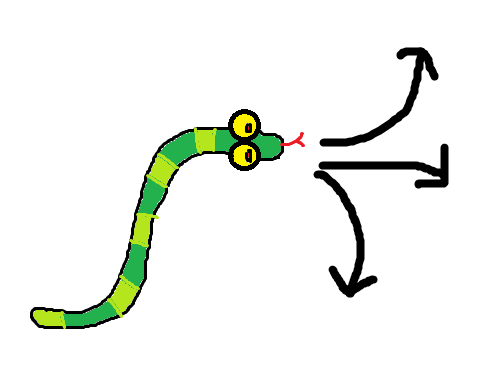
\includegraphics[scale=0.4]{ular-segala-arah}  
	\caption[Pergerakan ular ke segala arah]{Pergerakan ular ke segala arah} 
	\label{fig:ularSegalaArah} 
\end{figure} 

Permainan \textit{Snake} ini dapat dimainkan secara \textit{singleplayer} atau \textit{multiplayer}. \textit{Singleplayer game} adalah permainan yang dapat dimainkan oleh 1 pemain. \textit{Multiplayer game} adalah permainan yang dapat dimainkan oleh beberapa pemain. Pada umumnya, permainan \textit{Snake} dimainkan secara \textit{singleplayer}. Contoh \textit{singleplayer game Snake} adalah \textit{Snake} pada telepon genggam \textit{Nokia} yang dapat dilihat pada Gambar~\ref{fig:nokiaSnake}\footnote{https://en.wikipedia.org/wiki/Snake\_(video\_ game\_ genre)} dan contoh \textit{multiplayer game Snake} adalah \textit{Slither.io} yang dapat dilihat Gambar~\ref{fig:slither}\footnote{https://play.google.com/store/apps/details?id=air.com.hypah.io.slither}. \textit{Snake} dapat dimainkan menggunakan \textit{smartphone} dan \textit{web browser}.  

\begin{figure}[H]
	\centering  
	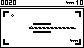
\includegraphics[scale=2]{nokiaSnake}  
	\caption[Permainan Snake pada telepon genggam \textit{Nokia}]{Permainan Snake pada telepon genggam \textit{Nokia}} 
	\label{fig:nokiaSnake} 
\end{figure} 

\begin{figure}[H]
	\centering  
	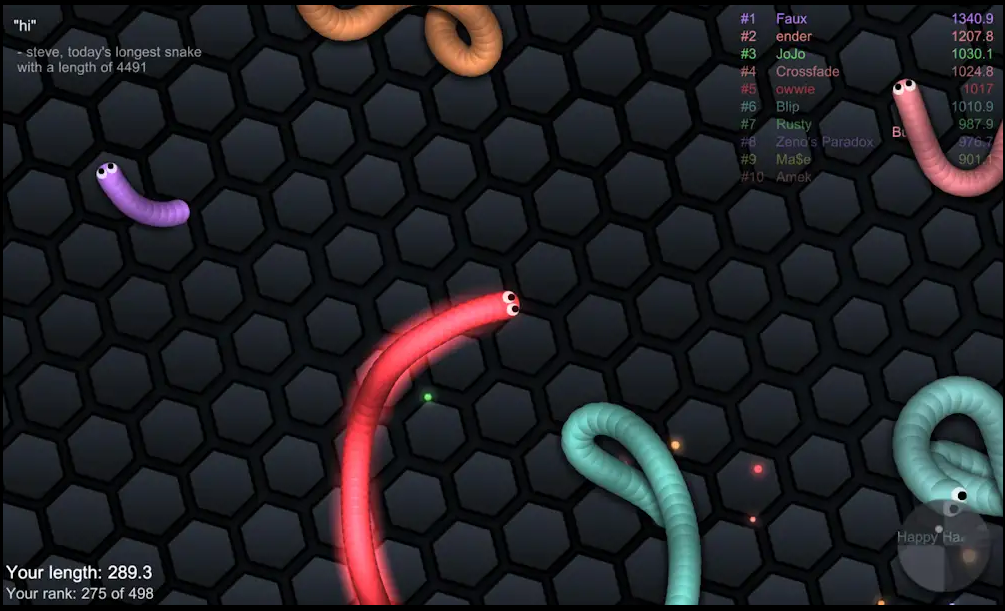
\includegraphics[scale=0.3]{slither}  
	\caption[Permainan \textit{Slither.io} pada \textit{Android}]{Permainan \textit{Slither.io} pada \textit{Android}} 
	\label{fig:slither} 
\end{figure} 

\section{HTML5 \textit{Canvas}}
\label{sec:HTML5Canvas}
HTML5 Canvas adalah sebuah daerah \textit{bitmap} yang dapat dimanipulasi oleh \textit{Javascript}. Pada daerah \textit{bitmap} tersebut, \textit{pixel-pixel} akan di\textit{render} oleh canvas. Setiap \textit{frame}, HTML5 Canvas akan menggambar pada area \textit{bitmap} tersebut menggunakan \textit{Canvas} API(\textit{Application Programming Interface}) yang dipanggil pada \textit{Javascript}. API dari HTML5 Canvas yang umum adalah 2D \textit{Context}. Dengan adanya 2D \textit{Context}, \textit{programmer} dapat membuat bentuk 2D, menampilkan gambar, \textit{render} tulisan, memberi warna, membuat garis dan kurva, dan manipulasi \textit{pixel}. HTML5 Canvas tidak hanya digunakan untuk menggambar dan menampilkan gambar serta tulisan. HTML5 Canvas dapat digunakan untuk membuat animasi, aplikasi pada \textit{web} dan permainan. 

Untuk menambahkan \textit{canvas} pada halaman HTML, diperlukan \textit{tag} <canvas>. Di bawah ini adalah potongan kode untuk menambahkan \textit{canvas} pada halaman HTML. 

\begin{lstlisting}[language=HTML, caption=Menambahkan \textit{canvas}]
	<canvas id='canvas' width='500' height='300'>
		Your browser does not support HTML5 Canvas.
	</canvas>
	
\end{lstlisting}


Berikut adalah penjelsan atribut yang ada pada \textit{canvas} berdasarkan potongan kode di atas : 
\begin{itemize}
	\item id
\end{itemize}


\section{\textit{\textit{Javascript}}}
\label{sec:Javascript}
\textit{Javascript} adalah bahasa pemrograman yang ringan, \textit{interpreted} dan berorientasi objek yang digunakan pada halaman \textit{web}. \textit{Javascript} dapat membuat objek dengan menambahkan \textit{method} dan atributnya sama seperti bahasa pemrograman C++ dan \textit{Java}. Setelah objek diinisialisasi, maka objek tersebut dapat dijadikan \textit{blueprint} untuk membuat objek lain yang mirip\footnote{https://developer.mozilla.org/en-US/docs/Web/JavaScript/About\_ JavaScript}. \textit{Javascript} dapat digunakan untuk mengimplementasi hal yang kompleks pada halaman web. Contohnya adalah menamplikan peta yang interaktif dan membuat animasi 2D/3D. Selain \textit{Javascript}, HTML(\textit{HyperText Markup Language}) dan CSS(\textit{Cascading Style Sheet}) merupakan bagian/komponen penting dalam pembuatan halaman \textit{web}\footnote{https://developer.mozilla.org/en-US/docs/Learn/JavaScript/First\_ steps/What\_ is\_ JavaScript}.\\


\subsection{Variabel}
Variabel adalah sebuah wadah untuk menyimpan nilai/\textit{value}. Untuk mendeklarasi variable pada \textit{Javascript}, digunakan \textit{keyword 'var'}. Variabel pada Javascript tidak perlu menuliskan tipe datanya ketika mendeklarasikan variabel. Di bawah ini adalah potongan kode untuk mendeklarasikan variabel.\footnote{https://developer.mozilla.org/en-US/docs/Web/JavaScript/Guide/Grammar\_ and\_ types}

\begin{lstlisting}[language=Javascript, caption=Deklarasi variabel]
	var myVariable;
	
\end{lstlisting}

Nilai variabel pada potongan kode di atas adalah \textit{undifined} karena variabel tersebut tidak diberi nilai/value. Di bawah ini adalah potongan kode untuk mengisi nilai pada variabel. 

\begin{lstlisting}[language=Javascript, caption=Mengisi nilai sebuah variabel]
	myVariable = 3;	
	
\end{lstlisting}

Variabel dapat menyimpan beberapa tipe data diantaranya adalah\footnote{https://developer.mozilla.org/en-US/docs/Learn/Getting\_ started\_ with\_ the\_ web/JavaScript\_ basics} :
\begin{itemize}
	\item \textit{String} : nilai yang berupa teks atau sekumpulan huruf.
	\item \textit{Number} : nilai yang berupa angka.
	\item \textit{Boolean} : nilai \textit{true/false}.
	\item \textit{Array} : struktur untuk menyimpan lebih dari 1 nilai dalam sebuah \textit{reference}
	\item \textit{Object} : semua yang ada pada Javascript termasuk objek pada HTML.
\end{itemize}

\subsection{\textit{Constant}}
\textit{Constant} adalah sebuah variabel \textit{read-only}, artinya nilai pada \textit{constant} tidak dapat diubah. Untuk mendeklarasikan \textit{constant}, digunakan \textit{keyword 'const'}. Di bawah ini adalah potongan kode untuk mendeklarasi \textit{constant}.

\begin{lstlisting}[language=Javascript, caption=Deklarasi \textit{constant}]
	const myConst = 1;
	
\end{lstlisting}

\subsection{\textit{Function}}
\textit{Function} adalah sekumpulan perintah/\textit{statements} untuk menjalankan suatu tugas atau menghitung nilai. Untuk membuat \textit{function}, digunakan \textit{keyword 'function'}, kemudian diikuti dengan nama \textit{function} tersebut, parameter yang dituliskan di dalam kurung, dan \textit{statement}/perintah \textit{Javascript} yang ditulis di dalam kurung kurawal. Parameter pada \textit{function} bisa lebih dari 1 yang penulisanya dipisahkan oleh tanda koma (,). \textit{Function} bisa memiliki parameter atau tidak. Di bawah ini adalah potongan kode untuk membuat \textit{function} penjumlahan 2 buah bilangan.

\begin{lstlisting}[language=Javascript, caption=\textit{Function} penjumlahan 2 buah bilangan]
	function penjumlahan(angka1,angka2){
		var hasil = angka1+angka2;
		return hasil;
	}
	
\end{lstlisting}

Setelah membuat \textit{function}, \textit{function} tersebut tidak langsung dieksekusi. Membuat \textit{function} hanya memberi nama \textit{function} tersebut dan mendeskripsikan apa yang akan dilakukan oleh \textit{function} tersebut apabila dipanggil. Dengan memanggil \textit{function}, maka \textit{function} akan dieksekusi\footnote{https://developer.mozilla.org/en-US/docs/Web/JavaScript/Guide/Functions}. Di bawah ini adalah potongan kode untuk memanggil \textit{function} dengan nama penjumlahan.

\begin{lstlisting}[language=Javascript, caption=Memanggil \textit{function} penjumlahan]
	penjumlahan(10,5);
	
\end{lstlisting}

\subsection{Menggambar pada \textit{Canvas}}
Sesudah menuliskan \textit{tag} <canvas> pada HTML, canvas tidak bisa langsung digambar. Karena itu perlu ditambahkan \textit{drawing context} pada \textit{Javascript}. Di bawah ini adalah potongan kode untuk menambahkan \textit{drawing context}.

\begin{lstlisting}[language=Javascript, caption=Menambahkan \textit{drawing context canvas}]
	var myCanvas = document.getElementById('canvas');
	var context = myCanvas.getContext('2d');
\end{lstlisting}

Berdasarkan potongan kode di atas, variabel myCanvas menyimpan objek dengan id = 'canvas'. Id ini mengacu ke objek \textit{canvas} pada HTML yang memilki id bernama canvas. Variabel myCanvas sekarang sudah menyimpan objek \textit{canvas}. Kemudian variabel context menyimpan \textit{drawing context} 2D. Sesudah itu, \textit{canvas} tersebut dapat digambar dengan bentuk 2D, garis, kurva, membuat tulisan, dan menambahkan gambar. Selain untuk menggambar, bentuk-bentuk tersebut dapat diberi warna sesuai dengan keinginan.\\

Untuk menggambar bentuk 2D atau garis, diperlukan koordinat x dan y. Koordinat tersebut akan menempatkan gambar tersebut pada \textit{canvas}. Posisi awal/\textit{origin} pada \textit{canvas} adalah (0,0) yang terletak di ujung kiri atas \textit{canvas}. Gambar~\ref{fig:grid}\footnote{https://developer.mozilla.org/en-US/docs/Web/API/Canvas\_ API/Tutorial/Drawing\_ shapes} adalah penempatan kotak biru pada \textit{canvas} terhadap \textit{origin}.

\begin{figure}[H]
	\centering  
	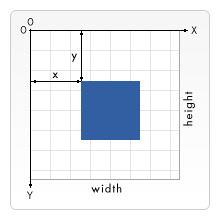
\includegraphics[scale=0.5]{grid}
	\caption[Posisi kotak biru pada \textit{canvas} terhadap \textit{origin}]{Posisi kotak biru pada \textit{canvas} terhadap \textit{origin}}
	\label{fig:grid} 
\end{figure} 

Pada di atas, titik ujung kiri kotak biru tersebut berjarak x \textit{pixel} dari kiri dan berjarak y \textit{pixel} dari atas. 

\subsubsection{Menggambar Persegi Panjang}
Ada 3 cara untuk menggambar persegi panjang:

\begin{itemize}
	\item \textit{fillRect(x,y,width,height)} : menggambar persegi panjang serta mengisi bagian tengah persegi panjang.
	\item \textit{strokeRect(x,y,width,height)} : menggambar \textit{outline} yang berbentuk persegi panjang.
	\item \textit{clearRect(x,y,width,height)} : menghapus daerah yang ditentukan pada \textit{canvas}. Daerah yang dihapus berbentuk persegi panjang.
\end{itemize}

Fungsi tersebut memiliki parameter yang sama. Parameter x dan y untuk menentukan posisi pada canvas dari titik ujung kiri atas persegi panjang. \textit{Width} adalah lebar dari persegi panjang dan \textit{height} adalah tinggi dari persegi panjang.

\subsubsection{Menggambar \textit{Path}}
\textit{Path} adalah sekumpulan titik yang dihubungkan oleh segmen garis. \textit{Path} dapat membentuk kurva dan membuat bentuk 2D lainnya seperti segitiga, trapesium, belah ketupat dan lain-lain. Langkah-langkah untuk membuat bentuk menggunakan path adalah sebegai berikut : 

\begin{enumerate}
	\item Buat \textit{path}.
	\item Tuliskan perintah untuk menggambar pada \textit{path} tersebut.
	\item Sesudah \textit{path} tersebut sudah dibuat, \textit{path} tersebut dapat di\textit{render} menggunakan \textit{stroke} atau \textit{fill}.
\end{enumerate}

Langkah pertama untuk membuat \textit{path} baru adalah dengan menggunakan fungsi \textit{beginPath()}. Setelah itu, perintah-perintah untuk menggambar dapat digunakan untuk membuat bentuk-bentuk yang diinginkan. Apabila sudah selesai menggambar, gunakan fungsi \textit{stroke()} untuk menggambar outline dari \textit{path} tersebut atau \textit{fill()} untuk mengisi area path tersebut. Setelah itu, gunakan fungsi \textit{closePath()} untuk menutup bentuk tersebut dengan cara menggambar garis lurus dari posisi titik terakhir ke titik awal. Fungsi lainnya yang menjadi bagian dari membuat \textit{path} adalah fungsi \textit{moveTo()}. Fungsi ini diibaratkan seperti mengangkat sebuah pensil dari sebuah titik pada kertas kemudian menempatkanya pada titik yang diinginkan. Di bawah ini adalah fungsi moveTo().

\begin{lstlisting}[language=Javascript, caption=Fungsi \textit{moveTo()}]
	moveTo(x,y);
\end{lstlisting}

Fungsi \textit{moveTo} memiliki 2 parameter yaitu x dan y yang merupakan posisi titik pada \textit{canvas}. Ketika canvas sudah diinisialsasi dan fungsi beginPath() sudah dipanggil, fungsi moveTo() berguna sebagai penempatan titik awal untuk menggambar. Fungsi lineTo() digunakan untuk menggambar sebuah garis. Di bawah ini adalah fungsi lineTo().

\begin{lstlisting}[language=Javascript, caption=Fungsi \textit{lineTo()}]
	lineTo(x,y);
\end{lstlisting}

Fungsi lineTo() memiliki 2 parameter yaitu x dan y yang merupakan titik akhir dari garis. Garis akan digambar mulai dari posisi titik awal sampai ke posisi titik akhir garis. Titik awal ini bergantung pada titik akhir dari \textit{path} sebelumya. Titik awal dapat diubah dengan menggunakan fungsi \textit{moveTo()}.

Fungsi \textit{arc()} digunakan untuk menggambar lingkaran atau busur. Di bawah ini adalah fungsi arc().

\begin{lstlisting}[language=Javascript, caption=Fungsi \textit{arc()}]
	arc(x,y,radius,startAngle,endAngle,anticlockwise);
\end{lstlisting}

Parameter x dan y adalah posisi titik tengah busur pada canvas. Radius adalah besar jari-jari busur. StartAngle dan endAngle adalah titik awal dan titik akhir busur dalam satuan radian yang diukur dari sumbu x. Anticlockwise adalah parameter yang bernilai boolean, apabila bernilai true, maka busur akan digambar berlawanan arah jarum jam dan jika bernilai false, busur akan digambar searah jarum jam. Karena fungsi arc() menerima input sudut dalam radian, maka perlu dilakukan konversi dari satuan derajat menjadi radian terlebih dahulu. Rumusnya adalah sebagai berikut :


\subsection{Membuat Objek pada \textit{Javascript}}


\subsection{\textit{Events}}


\subsection{Membuat Animasi}

\section{\textit{jQuery}}
\textit{jQuery} adalah pustaka yang dimiliki oleh \textit{Javascript}. Semua perintah-perintah pada \textit{Javascript} dapat digunakan oleh \textit{jQuery}. Penulisan \textit{jQuery} lebih singkat dibandingkan \textit{Javascript}.

Di bawah ini adalah potongan kode pada \textit{jQuery}. Untuk mendapatkan objek pada \textit{jQuery} selalu diawali dengan simbol '\$'. Kemudian diikuti dengan objeknya lalu \textit{method}nya. 

\begin{lstlisting}
	$( "h1" ).remove();
	
\end{lstlisting}

\textit{jQuery} dapat mendeteksi apakah halaman \textit{web} sudah siap atau belum. Potongan kode di bawah ini adalah untuk mendeteksi halaman \textit{web}.

\begin{lstlisting}
	$( document ).ready(function() {
    	// kode dituliskan di sini
	});
	
\end{lstlisting}

Kode yang dituliskan di dalam \$( document ).ready(function() akan dijalan setelah DOM(\textit{Document Object Model}) pada halaman web tersebut sudah siap untuk dieksekusi oleh \textit{Javascript}. 

\section{\textit{Git}}
\label{sec:Git}
\textit{Github} adalah layanan \textit{web hosting} bersama untuk proyek pengembangan perangkat lunak yang menggunakan sistem \textit{version control} yaitu \textit{Git}\footnote{https://en.wikipedia.org/wiki/GitHub}. \textit{Git} dapat mengetahui perubahan pada file di komputer. \textit{Github} biasanya digunakan oleh para \textit{programmer} untuk menambahkan/merevisi \textit{source code} dan sebagai media untuk berkolaborasi dalam proyek pembangunan perangkat lunak. \textit{Source code} tersebut disimpan dikelompokan pada file dan file tersebut disimpan di\textit{repository}. Dalam 1 \textit{repository}, \textit{owner}(pengguna yang membuat \textit{repository}) dapat mengundang pengguna lain untuk berkolaborasi. Ketika ada perubahan pada \textit{repository}, maka \textit{collaborator}(pengguna yang diberi hak untuk mengubah \textit{repository}) dapat mengetahui \textit{source code} atau file yang direvisi oleh \textit{collaborator} lain.\\

\textit{Github} memiliki banyak fitur untuk memudahkan kerja \textit{programmer}. Fitur \textit{Github} yang mendukung penelitian ini adalah \textit{pull request}. \textit{Pull request} memberitahu \textit{collaborator} lain tentang perubahan pada \textit{repository}. Dengan adanya \textit{pull request}, pengguna dan \textit{collaborator} lain dapat berdiskusi tentang perubahan tersebut. Perubahan tersebut harus di \textit{merge} oleh \textit{collaborator} dari \textit{repository}. Apabila sudah di \textit{merge} oleh \textit{collaborator}, perubahan tersebut akan disimpan di \textit{repository}\footnote{https://help.github.com/articles/about-pull-requests}.